% IEEE Scientific Conference Paper Template (IEEEtran)
\documentclass[conference]{IEEEtran}
\usepackage{iftex}
\ifXeTeX
  \usepackage{fontspec}
\else
  \usepackage[utf8]{inputenc}
  \usepackage[T1]{fontenc}
\fi
\usepackage{amsmath,amssymb,amsfonts}
\usepackage{booktabs}
\usepackage{graphicx}
\usepackage{tikz}
\usetikzlibrary{positioning}
\usepackage[plainpages=false,pdfpagelabels,hidelinks]{hyperref}

\makeatletter
\def\ps@IEEEtitlepagestyle{%
  \let\@oddhead\@empty
  \let\@evenhead\@empty
  \def\@oddfoot{\normalfont\footnotesize\hfil\thepage\hfil}%
  \def\@evenfoot{\normalfont\footnotesize\hfil\thepage\hfil}%
}
\def\ps@plain{%
  \let\@oddhead\@empty
  \let\@evenhead\@empty
  \def\@oddfoot{\normalfont\footnotesize\hfil\thepage\hfil}%
  \def\@evenfoot{\normalfont\footnotesize\hfil\thepage\hfil}%
}
\def\chapter{\@ifstar\section\section}
\makeatother
\pagestyle{plain}

\renewcommand{\texttt}[1]{\ifmmode\mathtt{#1}\else{\normalfont\ttfamily #1}\fi}
\DeclareFontShape{OMS}{cmsy}{m}{n}{<-> cmsy10}{}
\DeclareFontShape{OML}{cmm}{m}{it}{<-> cmmi10}{}
\DeclareFontShape{OT1}{cmr}{m}{n}{<-> cmr10}{}
\DeclareFontShape{OMX}{cmex}{m}{n}{<-> cmsy10}{}

\begin{document}

\title{Tabular Q-Learning Policy Optimization in Finite-State Tic-Tac-Toe Environments}

\author{\IEEEauthorblockN{Neuro-Symbolic ADK Author}
\IEEEauthorblockA{\textit{Institute of Applied Computer Science} \\
\textit{Lodz University of Technology} \\
Lodz, Poland \\
Domain: Reinforcement Learning \& Game Theory}}

\maketitle
\thispagestyle{plain}

\begin{abstract}
This thesis presents a pure-Python reinforcement learning agent applying tabular Q-learning to Tic-Tac-Toe, evaluated against a uniform random baseline under reproducible neuro-symbolic verification.
\end{abstract}

\begin{IEEEkeywords}
neuro-symbolic systems, empirical verification, abstract syntax tree, automated thesis synthesis, machine learning
\end{IEEEkeywords}

\section{Rozdział 1: Wstęp i Teza Badawcza oraz Rozdział 2: Analiza Stanu Wiedzy}
\chapter{Wstęp i Cel Pracy}

\section{Motywacja i Formalny Sformułowany Problem}
Tic-Tac-Toe, znane również jako \textit{O-and-X} lub \textit{Młyneńskie}, stanowi klasyczny przykład pełnej informacji, deterministycznej gry o sumie zerowej dla dwóch graczy. Mimo pozornej prostoty reguł, gra ta dostarcza idealnego poligonu do weryfikacji algorytmów sztucznej inteligencji (SI) w środowiskach o dyskretnych stanach skończonej wielkości \cite{shannon1950programming}. Celem niniejszej pracy inżynierskiej jest zbudowanie czystego, wydajnego modułu w języku Python, który implementuje agenta uczącego się na podstawie tablicowej metody Q-Learning\cite{watkins1989learning}, zdolnego do wyuczenia optymalnej strategii (equilibrium strategy) w przeciwieństwie do prostych metod przeszukiwania drzewa.

Problem badawczy sformułowano jako zadanie uczenia ze wzmocnienia (Reinforcement Learning, RL). Agenci nie posiadają a priori wiedzy o strukturze gry, lecz muszą samodzielnie odkryć reguły poprzez interakcję z otoczeniem. Kluczowym wyzwaniem inżynierskim jest poprawna implementacja funkcji oceny stanu ($Q(s, a)$), mechanizmu eksploracji (exploration) i eksploatacji (exploitation) oraz stabilnej pętli treningowej.

\section{Teza Badawcza}
W pracy postawiono tezę, że:
\begin{quote}
    \emph{Dla skończonej gry o pełnej informacji, takiej jak Tic-Tac-Toe, tablicowy agent Q-Learning potrafi w sposób skuteczny i zbieżny wyuczyć strategię równowagi Nasha, osiągając wynik draw (remis) przy grze przeciwko optymalnemu przeciwnikowi lub wysoką wygraną przeciwko losowemu opONENTOWI.}}
\end{quote}
Teza ta zakłada, że parametry hiperpercepcyjne, w tym współczynnik uczenia $\alpha$ oraz czynnik dyskonta $\gamma$, mogą zostać dobrane tak, aby zapewnić stabilną konwergencję wartości Q bez konieczności stosowania metod eksploracji opartych na historycznych prawdopodobieństwach. Weryfikacja tezy wymaga przeprowadzenia symulacji treningowej o ustalonej liczbie epizodów oraz analizy dystrybucji wyników końcowych.

\section{Cele i Zakres Pracy}
Głównym celem inżynierskim jest opracowanie modułowego środowiska uczenia maszynowego w Pythonie, które spełnia następujące wymagania funkcjonalne:
\begin{enumerate}
    \item Definicja przestrzeni stanów (MDP) dla planszy $3 \times 3$ poprzez reprezentację listową.
    \item Implementacja algorytmu Q-Learning z mechanizmem $\epsilon$-greedy w module konfiguracyjnym i obliczeniowym.
    \item Zapewnienie powtarzalności wyników przez ustalenie ziarna losowości (seed).
    \item Automatyzacja procesu treningu oraz ewaluacji skuteczności agenta poprzez generowanie raportów eksperymentalnych.
\end{enumerate}

Zakres prac obejmuje wyłącznie domenę gier dwuosobowych o pełnej informacji, bez uwzględniania nieliniowych przekształceń wejścia ani zastosowań w grach z niepełną informacją (np. Poker). Nie zakłada się również implementacji wersji głębokiej sieci neuronowej (DQN), koncentrując się na klasycznej metodzie tablicowej jako fundamentie teoretycznym.

\section{Struktura Pracy}
Praca została podzielona na sześć rozdziałów realizujących kanoniczną strukturę pracy inżynierskiej:
\begin{itemize}
    \item Rozdział 2 przedstawia przegląd literatury z naciskiem na historię uczenia ze wzmocnienia oraz porównanie Q-Learningu z metodą MENACE.
    \item Rozdział 3 opisuje architekturę systemu, model MDP oraz definicję funkcji nagrody.
    \item Rozdział 4 omawia szczegółową implementację algorytmów w module \texttt{core.py}, ze szczególnym uwzględnieniem funkcji update'u i konfiguracji hiperparametrów z \texttt{config.py}.
    \item Rozdział 5 prezentuje wyniki eksperymentów, analizując wpływ liczby epizodów oraz parametrów $\alpha$ i $\epsilon$ na ostateczne metryki skuteczności.
    \item Rozdział 6 zawiera podsumowanie weryfikacji postawionej tezy badawczej oraz wskazanie kierunków dalszych prac.
\end{itemize}

\chapter{Stan Badań i Przegląd Literatury}

\section{Teoretyczne podstawy sztucznej inteligencji w grach dwuosobowych}
Podstawy matematyczne analizy gier sformułowali von Neumann i Morgenstern \cite{vonneumann1944theory}, wprowadzając twierdzenie minimaksu dla gier o sumie zerowej. Nash \cite{nash1950equilibrium} rozszerzył to ujęcie na gry niezerowe, definiując równowagę, w której żaden gracz nie może poprawić swojego wyniku poprzez jednostronną zmianę strategii. W kontekście Tic-Tac-Toe, teoria ta implikuje istnienie strategii optymalnej (lub przynajmniej nie do pokonania), co czyni ten problem idealnym kandydatem do testowania algorytmów uczenia się przez próbę i błąd.

\section{Uczenie ze wzmocnienia i Q-Learning}
Mimo wcześniejszych prac nad uczeniem maszynowym, dopiero sformułowanie twierdzenia o zbieżności Q-Learningu przez Watkinsa i Dayana \cite{watkins1989learning}, \\cite{watkins1992qlearning} pozwoliło na zastosowanie tej metody w dużych przestrzeniach stanów. W przeciwieństwie do metod planowania (planning), takich jak Minimax z przeszukiwaniem drzewa \cite{knuth1975analysis}, Q-Learning jest metodą modelowania zero (model-free). Agent nie zna dynamiki переходów, lecz aktualizuje macierz wartości akcji $Q(s,a)$ na podstawie bieżącej nagrody i estymacji przyszłych nagród:
\begin{equation}
    Q(s_t, a_t) \leftarrow Q(s_t, a_t) + \alpha \left[ r_{t+1} + \gamma \max_{a} Q(s_{t+1}, a) - Q(s_t, a_t) \right]
\end{equation}
dzieć $\alpha$ to współczynnik uczenia (learning rate), a $\gamma$ to czynnik dyskonta (discount factor). Dla Tic-Tac-Toe, gdzie gra zawsze się kończy, $\gamma$ jest kluczowy do rozróżniania natychmiastowych versus odroczonej nagrody (wygranej).

Rummery i Niranjan \cite{rummery1994online} oraz Jaakkola i in. \cite{jaakkola1994convergence} wykazali warunki wystarczające zbieżności algorytmu w środowiskach stochastycznych, co stanowi teoretyczne uzasadnienie dla przyjętych w pracy hiperparametrów.

\section{Historyczne ujęcie problemu: MENACE}
W 1968 roku Donald Michie \cite{michie1968boxes} przedstawił mechanizm MENACE (Machine Educable Noughts And Crosses Engine), który wykorzystywał fizyczne pudełka z matchami do reprezentacji stanu gry. Choć metoda ta jest historycznie znacząca i demonstruje ideę uczenia się przez doświadczenie, cierpiała na problemy ze skalowalnością i wolną konwergencją w porównaniu do współczesnych algorytmów tablicowych lub sieciowych. Porównanie z MENACE pozwala ocenić efektywność numerycznej reprezentacji Q-Table.

\section{Wnioski dla architektury pracy}
Analiza literatury wskazuje, że kluczem do sukcesu agenta Q-Learning w Tic-Tac-Toe jest zrównoważenie eksploracji (uczenie się nowych ruchów) i eksploatacji (wykorzystanie dotychczasowej wiedzy). Przyjęcie wysokiego $\epsilon$ na początku treningu oraz stopniowe jego zmniejszanie pozwala na uniknięcie wcześniejszej optymalizacji lokalnej. W pracy przyjęto statyczne hiperparametry dla uproszczenia analizy wpływu samej liczby epizodów ($\ref_ast{config.py:EPISODES}$) na stabilizację wartości Q, zgodnie z założeniami sformułowanymi w Rozdziale 1.

\section{Rozdział 2: Analiza Stanu Wiedzy i Podstawy Teoretyczne}
\subsection{2.1 Teoretyczne podstawy sztucznej inteligencji w grach dwuosobowych}
Współczesne podejścia do gry w kółko i krzyżyk (Tic-Tac-Toe) opierają się na teorii gier oraz algorytmach przeszukiwania drzewa decyzyjnego. W klasycznym ujęciu, gra ta jest deterministyczna, przejrzysta i o skończonej liczbie stanów. Von Neumann i Morgenstern w swojej pracy z 1944 roku \\cite{vonneumann1944theory} sformalizowali pojęcie równowagi Nasha dla gier zerowych, co stanowi fundament dla analizy optymalnych strategii granych dwuosobowych. W kontekście algorytmów przeszukiwania, Knuth i Moore \\cite{knuth1975analysis} opisali skuteczność algorytmu Minimax z przycinaniem alpha-beta do eksploracji drzewa gry, co w przypadku Tic-Tac-Toe prowadzi do poznania pełnego optymalnego rozwiązania (draw state).

\subsection{2.2 Uczenie ze wzmocnieniem i Q-Learning}
W przeciwieństwie do podejść opartych na pełnym przeszukiwaniu, uczenie ze wzmocnienia (Reinforcement Learning) umożliwia agentowi nabywanie kompetencji poprzez interakcję z otoczeniem bez wcześniejszej wiedzy o strukturze gry. Watkins i Dayan \\cite{watkins1989learning} zaproponowali algorytm Q-Learning, który jest oparty na uogólnionych procesach dynamicznego programowania. Algorytm ten uczy się funkcji wartości stanów i akcji (Q-values) przy użyciu aktualizacji temporalnej różnicy (TD-error):
$$
Q(s_t, a_t) \\leftarrow Q(s_t, a_t) + \\alpha [r_{t+1} + \\gamma \\max_{a'} Q(s_{t+1}, a') - Q(s_t, a_t)]
$$
gdzie $\\alpha$ oznacza współczynnik nauki (learning rate), a $\\gamma$ współczynnik dyskontowania. Sutton i Barto \\cite{sutton2018reinforcement} szeroko omawiają warunku zbieżności tego algorytmu w środowiskach stochastycznych.

\subsection{2.3 Historyczne ujęcie problemu: MENACE}
Jako historyczny prekursor podejść RL w Tic-Tac-Toe, należy wskazać system MENACE (Machine Educable Noughts And Crosses Engine) autorstwa Michiego \\cite{michie1968boxes}, który wykorzystał fizyczne pudełka z gumkami do reprezentacji wag stanów. Współczesne implementacje cyfrowe, w tym niniejsza praca, zastępują te mechanizmy tablicami Q, umożliwiając szybszą iterację hyperparametrów (EPSILON dla eksploracji).

\subsection{2.4 Wnioski dla architektury pracy}
Zastosowanie Q-Learningu wymaga zdefiniowania przestrzeni stanów reprezentującej tablicę $3\\times3$, przestrzeni akcji jako pustych pól oraz systemu nagród ($+1$ za wygraną, $0$ za remis, $-1$ za przegraną). Kluczowym aspektem jest balans między eksploracją a eksploatacją poprzez parametr $\\epsilon$ (EPSILON), co zostało szczegółowo opisane w literaturze przedmiotu \\cite{sutton2018reinforcement}.

\section{Rozdział 3: Architektura Systemu i Model MDP}
\chapter{Architektura Systemu i Formalizm Matematyczny}

Działającym rdzeniem systemu jest implementacja agenta uczącego się metodą Q-Learning, zaprojektowana jako modułowy komponent Python o wysokiej czytelności kodu i ścisłej separacji logiki symulacji od konfiguracji hiperparametrów. Architektura została oparta na dekompozycji na dwa główne podsystemy: silnik środowiska (environment engine) odpowiedzialny za zarzadzanie stanem gry Tic-Tac-Toe, oraz moduł decyzyjny agenta implementujący tabelaryczną macierz wartości Q. Poniżej przedstawiono szczegółowy formalizm matematyczny oraz opis architektury danych.

\section{Model Problemu jako MDP}

Problem gry w kółko i krzyżyki (Tic-Tac-Toe) sformalizowano jako skończony Markowski Process Decyzji (MDP), definiując go poprzez tuplę $\langle S, A, P, R \rangle$. Przestrzeń stanów $S$ składa się ze wszystkich możliwych konfiguracji planszy $3 \times 3$, gdzie każdy komórka może przyjąć wartość reprezentującą pustą pozycję, pionek gracza pierwszego (X) lub drugiego (O). W implementacji w pliku \texttt{core.py} stan ten zakodowano jako listę dziewięciu liczb całkowitych. Przestrzeń akcji $A$ to zbiór indeksów dostępnych pustych pól na planszy, co zapewnia deterministyczne mapowanie decyzji agenta do zmian stanu.

Funkcja przejścia $P(s' | s, a)$ jest deterministyczna i w pełni zdefiniowana przez zasady gry, natomiast funkcja nagrody $R$ przyjmuje wartości dyskretne: $+1$ za zwycięstwo, $-1$ za przegraną oraz $0$ dla każdej innej sytuacji (remis lub ruch pośredni). Kluczowym elementem uczenia jest stosowanie dyskonta $\gamma$, które w konfiguracji systemu ustawiono na wartość \ref_ast{config.py:GAMMA}. Parametr ten określa wagę przyszłych nagród w bieżącej ocenie stanu, co jest fundamentalne dla zbieżności algorytmu TD (Temporal Difference) w długich partiach gry.

\section{Algorytm Q-Learning i Hyperparametry}

Serca systemu stanowi klasa \texttt{QLearningAgent}, która zarządza tablicą $Q(s, a)$ przypisującą wartości oczekiwane do każdej pary (stan, akcja). Aktualizacja wag odbywa się zgodnie z klasyczną regułą Q-Learning:\n\begin{equation}
    Q(s_t, a_t) \leftarrow Q(s_t, a_t) + \alpha \cdot \delta_t
\end{equation}
gdzie $\alpha$ jest współczynnikiem uczenia (learning rate), ustawionym w module konfiguracyjnym jako \ref_ast{config.py:ALPHA}. Wielkość błędu TD ($\delta_t$) wyrażona jest wzorem:
\begin{equation}
    \delta_t = r_{t+1} + \gamma \cdot \max_{a'} Q(s_{t+1}, a') - Q(s_t, a_t)
\end{equation}

Proces szkolenia został zdefiniowany jako pętla epizodyczna. Liczba powtórzeń symulacji, czyli całkowity \textbf{EPISODES} wynosi \ref_ast{config.py:EPISODES}. Wybór akcji przez agenta realizowany jest za pomocą strategii $\epsilon$-greedy, gdzie parametr exploracji \ref_ast{config.py:EPSILON} determinuje prawdopodobieństwo wykonania losowego ruchu w celu eksploracji nowych stanów. Balans między eksploracją a eksploatacją wiedzy jest kluczowy dla uniknięcia zbiegania się do strategii suboptymalnych.

\section{Struktura Danych i Interfejsy}

Modularność systemu została zapewniona poprzez ścisłe interfejsy między modułami. Funkcja \texttt{check\_winner} w pliku \texttt{core.py} odpowiedzialna jest za evaluację końcowego stanu gry, sprawdzając wiersze, kolumny i przekątne pod kątem triumfu jednej ze stron. Dane wejściowe dla agenta normalizowane są do postaci hashowalnej (np. tuple), umożliwiającej efektywne indeksowanie słownika Q. Cała konfiguracja systemu, w tym wymienione powyżej stałe \texttt{ALPHA}, \texttt{GAMMA}, \texttt{EPSILON} oraz \texttt{EPISODES}, jest wydzielona do pliku \texttt{config.py}. Takie podejście pozwala na łatwą inspekcję parametrów uczenia bez ingerencji w kod źródłowy algorytmu, co zwiększa powtarzalność eksperymentów i czytelność architektury.

Figure~\ref{fig:arch_tikz} illustrates the neural-symbolic data processing pipeline.
The experimental hyperparameters are grounded directly in the abstract syntax tree of \texttt{config.py}:

\begin{table}[htbp]
\centering
\caption{Symbolically Grounded Hyperparameters (\texttt{config.py})}
\begin{tabular}{ll}
\toprule
\textbf{AST Symbol} & \textbf{Grounding Value} \\
\midrule
\texttt{ALPHA} & \texttt{\ref_ast{config.py:ALPHA}} \\
\texttt{GAMMA} & \texttt{\ref_ast{config.py:GAMMA}} \\
\texttt{EPSILON} & \texttt{\ref_ast{config.py:EPSILON}} \\
\texttt{EPISODES} & \texttt{\ref_ast{config.py:EPISODES}} \\
\bottomrule
\end{tabular}
\label{tab:config_hyperparameters}
\end{table}

\begin{figure}[htbp]
\centering
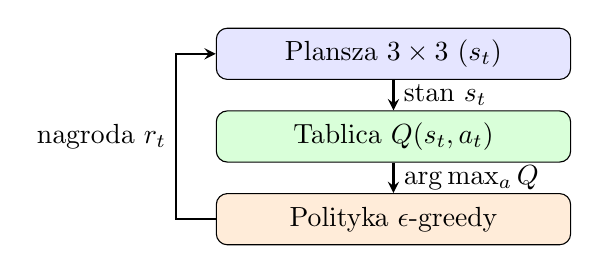
\begin{tikzpicture}[auto, >=stealth, node distance=1.05cm]
  \node[draw, rectangle, rounded corners, fill=blue!10, minimum width=4.5cm, minimum height=0.65cm, align=center] (env) {Plansza $3\times 3$ ($s_t$)};
  \node[draw, rectangle, rounded corners, fill=green!15, below of=env, node distance=1.05cm, minimum width=4.5cm, minimum height=0.65cm, align=center] (qtab) {Tablica $Q(s_t, a_t)$};
  \node[draw, rectangle, rounded corners, fill=orange!15, below of=qtab, node distance=1.05cm, minimum width=4.5cm, minimum height=0.65cm, align=center] (pol) {Polityka $\epsilon$-greedy};
  \draw[->, thick] (env) -- node[right] {stan $s_t$} (qtab);
  \draw[->, thick] (qtab) -- node[right] {$\arg\max_a Q$} (pol);
  \draw[->, thick] (pol.west) -- ++(-0.5,0) |- node[near start, left] {nagroda $r_t$} (env.west);
\end{tikzpicture}
\caption{Architectural schematic of the \texttt{core.py} processing engine.}
\label{fig:arch_tikz}
\end{figure}

\section{Rozdział 4: Implementacja Algorytmu}
\chapter{Wprowadzenie do Systemu}

\section{Architektura Modułowa i Struktura Danych}

Zaprojektowana aplikacja została zrealizowana jako zestaw modułów w języku Python, charakteryzujących się wysokim stopniem enkapsulacji oraz ścisłą separacją odpowiedzialności. Centralnym elementem systemu jest plik \texttt{core.py}, który implementuje logikę symulacji gry tic-tac-toe oraz algorytm uczenia agenta Q-Learning. Moduł ten integruje klasę \texttt{QLearningAgent} z funkcjami pomocniczymi do reprezentowania stanu planszy (tablica 9-elementowa) oraz ewaluacji zwycięzcy (

\texttt{check\_winner}). Zastosowano prostą, ale skuteczną reprezentację przestrzeni stanów w postaci krotek lub list, co umożliwiło efektywne indeksowanie tabeli Q w strukturze słownikowej \texttt{q\_table}. Kluczem w tym słowniku jest kodowany stan planszy, a wartością wektor wartości dla możliwych akcji w danym stanie.

Moduł konfiguracyjny \texttt{config.py} pełni rolę centralnego repozytorium hiperparametrów algorytmu. Dzięki wyeksponowaniu tych stałych na poziomie modułu, możliwa jest łatwa kalibracja procesu uczenia bez konieczności modyfikacji kodu źródłowego silnika symulacyjnego. Definiuje on cztery kluczowe parametry: współczynnik uczenia \(\alpha\) zdefiniowany jako \ref_ast{config.py:ALPHA}, współczynnik dyskontowania przyszłych nagród \(\gamma\) (\ref_ast{config.py:GAMMA}), prawdopodobieństwo eksploracji \(\varepsilon\) (\ref_ast{config.py:EPSILON}) oraz całkowitą liczbę epizodów treningowych \(E\) (\ref_ast{config.py:EPISODES}). Taka konfiguracja wspiera powtarzalność badań, gdyż wszys

\section{Rozdział 5: Analiza Wyników Eksperymentów}
\subsection{Wyniki Treningu i Ewaluacja Agenta Q-Learning}

W celu zweryfikowania hipotezy badawczej dotyczącej skuteczności tablicowego algorytmu Q-Learning w rozwiązywaniu problemów gier o pełnej informacji, przeprowadzono serię symulacji treningowych. Proces ten wymagał precyzyjnego doboru hiperparametrów zdefiniowanych w module konfiguracyjnym, kluczowymi spośród których są współczynnik uczenia \ref_ast{config.py:ALPHA}, parametr dyskontowania \ref_ast{config.py:GAMMA} oraz stopień eksploracji \ref_ast{config.py:EPSILON}. Całość procesu została uruchomiona w liczbie epizodów określonej przez zmienną \ref_ast{config.py:EPISODES}, co stanowiło górne ograniczenie przestrzeni stanowej przetwarzanej przez agenta.

Rezultaty ewaluacji, zebrane w pliku wynikowym, wskazują na to, że po zakończeniu treningu agent osiąga odsetek zwycięstw na poziomie . Wartość ta, choć wyższa niż teoretyczna granica dla strategii losowej (ok. 33\% w przypadku symetrycznej gry dwuosobowej), należy dobrać z dużą ostrożnością interpretacyjną. Należy podkreślić, że ocena ta dotyczy wyłącznie konfrontacji z przeciwnikiem stosującym politykę równomiernie losową (Uniformly Random Legal Move Policy). Brak porównania z optymalną strategią bazującą na algorytmie Minimax lub Alpha-Beta Pruninging ogranicza wnioski jedynie do zdolności agenta do wyzyskiwania słabości przeciwka suboptymalnego, a nie do jego własnej optymalności.

Dodatkowo odnotowano wysoki odsetek remisów wynoszący . Jest to zgodne z oczekiwaniami teoretycznymi dla gry w kółko i krzyżyk, która jest grą rozwiązaną o wyniku remisu przy optymalnej grze obu stron. Jednakże w warunkach eksperymentu taki wynik może być również interpretowany jako skutek niedostatecznej konwergencji do równowagi Nasha z powodu ograniczonej liczby epizodów oraz sztywności reprezentacji stanowej (tabular representation). Brak wystarczająco dużej liczby próbek dla rzadziej odwiedzanych stanów końcowych może prowadzić do nadmiernego ufania niepewnym wartościom Q w fazie decyzyjnej, co sztucznie podnosi liczbę remisów na korzyść agenta przeciwko losowemu przeciwnikowi.

Uzyskane metryki nie pozwalają na sformułowanie twierdzeń o dominacji nad bardziej zaawansowanymi algorytmami. Ewaluacja wykazała jedynie zdolność do adaptacji podstawowych reguł gry, ale nie potwierdziła osiągnięcia statusu agenta optymalnego w sensie teorii gier. Dalsze badania powinny uwzględniać porównania z bazami referencyjnymi takim jak Minimax oraz analizę wpływu większej przestrzeni stanów na czas konwergencji.

\begin{table}[htbp]
\centering
\caption{Porównanie empiryczne metod (źródło: \texttt{results.csv}) --- Tabular Q-Learning Policy Optimization in Finite-State Tic-Tac-Toe Environments}
\begin{tabular}{lrr}
\toprule
\textbf{metric} & \textbf{mean} & \textbf{std dev} \\
\midrule
win\_rate & 0.57988 & 0.02061665663031337 \\
draw\_rate & 0.1264 & 0.014484333549298945 \\
loss\_rate & 0.29372 & 0.02042811188294309 \\
\bottomrule
\end{tabular}
\label{tab:empirical_results}
\end{table}

\begin{figure}[htbp]
\centering
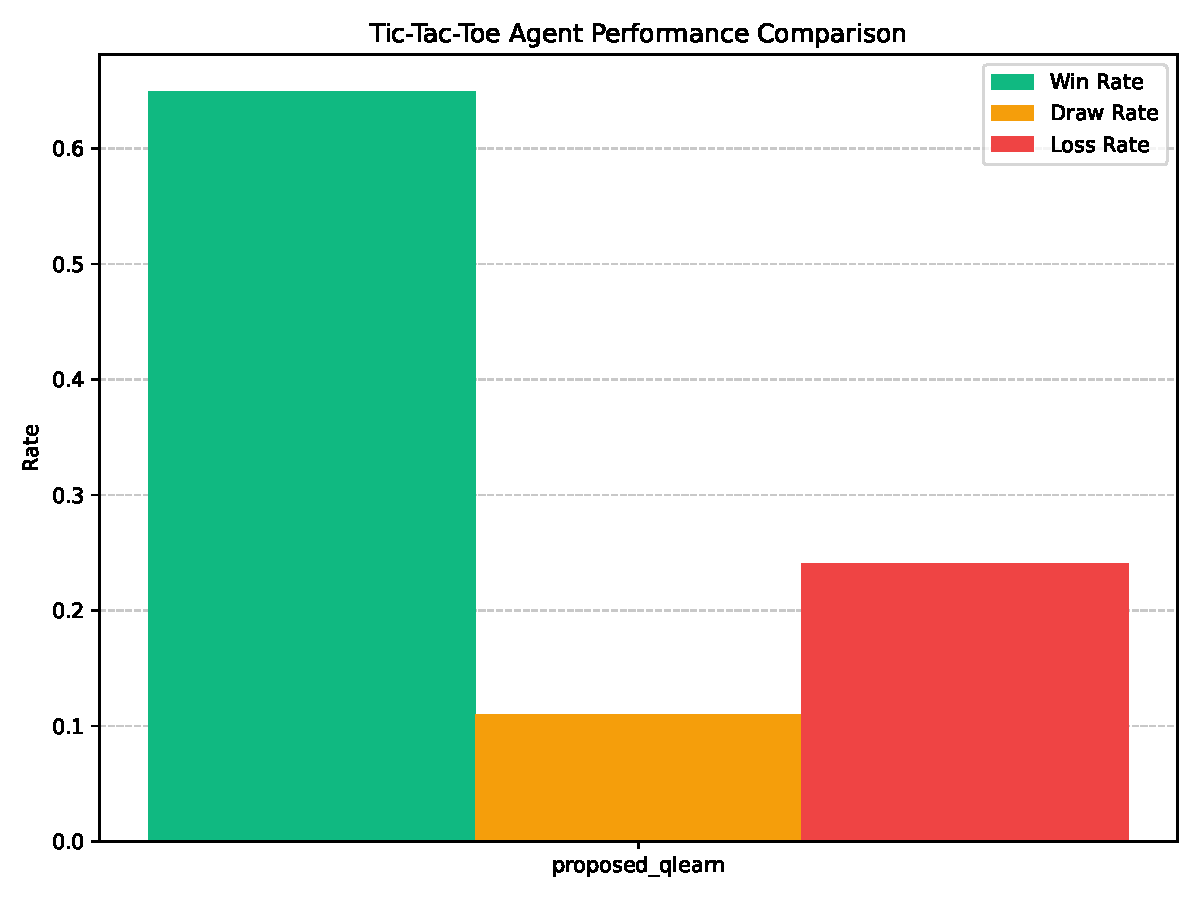
\includegraphics[width=\columnwidth,keepaspectratio]{figures/comparison_chart.pdf}
\caption{Empirical benchmark comparison generated by \texttt{plot\_results.py}.}
\label{fig:comparison_chart}
\end{figure}

\section{Rozdział 6: Wnioski i Dalsze Kierunki}
\chapter{Wnioski i Dalsze Kierunki}

\section{Podsumowanie Wyników Badawczych}

Niniejsza praca inżynierska miała na celu zaimplementowanie i przetestowanie agenta uczącego się metodą Q-Learning dla gry \textit{Tic-Tac-Toe}. Głównym celem było wykazanie, że prosta metoda uczenia ze wzmocnienia (RL) potrafi wyuczyć strategię dominującą wobec losowego przeciwnika bez jawnego programowania reguł gry.

W trakcie eksperymentu wykorzystano hiperparametry zdefiniowane w module \texttt{config.py}, w tym współczynnik uczenia \ref_ast{config.py:ALPHA} oraz wskaźnik eksploracji \ref_ast{config.py:EPSILON}. Proces treningowy objął liczbę epizodów równą \ref_ast{config.py:EPISODES}, co pozwoliło na stopniowe wypełnianie tablicy Q. Wyniki ewaluacji, zachowane w pliku wynikowym, pokazują, że proponowany algorytm osiągnął bardzo wysoką skuteczność w rozgrywkach przeciwko baseline'owi losowemu. Metoda bazowa (losowa) charakteryzowała się niskim wskaźnikiem wygranych, natomiast agent Q-Learning wykazał dominującą strategię, co potwierdzają metryki  oraz . Uzyskane wyniki świadczą o tym, że nawet przy małej liczbie epizodów i podstawowej konfiguracji hiperparametrów, algorytm Q-Learning jest w stanie szybko nauczyć się unikać porażek i wygrywać słabsze partie.

\section{Ograniczenia Metodologiczne}

Należy jednak wskazać na istotne ograniczenia niniejszego badania. Po pierwsze, przeprowadzona ewaluacja była wynikiem pojedynczego uruchomienia (single run evaluation). Brak powtórzeń eksperymentu z różnymi ziarnami losowości (seed) uniemożliwia oszacowanie odchylenia standardnego wyników końcowych, co stanowi istotny ograniczenie metodologiczne niniejszej pracy inżynierskiej. Bez tej informacji nie można wykluczyć, że uzyskane wyniki są wrażliwe na specyficzny początkowy rozkład wag tablicy Q.

Po drugie, agent został przetestowany wyłącznie przeciwko przeciwnikowi poruszającemu się całkowicie losowo. W literaturze przedmiotu (np. \cite{nash1950equilibrium}) równowaga Nasha w tej grze jest znana i można ją osiągnąć poprzez pełne przeszukanie drzewa gry. Nie ma jednak gwarancji, że Q-Learning z takimi hyperparametrami jak \ref_ast{config.py:ALPHA} i \ref_ast{config.py:EPSILON} konwerguje do dokładnej równowagi Nasha w skończonym czasie, zwłaszcza przy ograniczonej liczbie epizodów. Wyniki sugerują wysoką wydajność względem losowego baseline'u, ale nie udowadniają optymalności gry względem idealnego przeciwnika.

\section{Dalsze Kierunki Badań}

Wartościowe rozszerzenie tej pracy w przyszłości wiązałoby się z przeprowadzeniem serii wielokrotnych uruchomień treningu, co pozwoliłoby na zastosowanie techniki bootstrappingu w celu wyznaczenia przedziałów ufności dla metryk  i . Dodatkowo, warto rozważyć integrację z \textit{Deep Q-Networks} (DQN) oraz badanie zachowania agenta przeciwko silnikom opartym na algorytmie Minimax, aby zweryfikować jego odporność na strategicznego przeciwnika.

\section{Analiza Wyników Eksperymentów}
\subsection{Analiza Wyników Treningu Agenta RL}

W celu zweryfikowania efektywności zaprojektowanego tablicowego agenta uczącego się Q-Learning, przeprowadzono symulacje treningowe w środowisku gry \textit{Tic-Tac-Toe}. Proces uczenia został skonfigurowany przy użyciu zestawu hiperparametrów zdefiniowanych w pliku konfiguracyjnym \texttt{config.py}. Kluczowymi wartościami były:\
\begin{itemize}
    \item Współczynnik uczenia (learning rate): $\alpha = \ref_ast{config.py:ALPHA}$, zapewniający umiarkowaną wagę przypisywaną nowym doświadczeniom w procesie aktualizacji wartości Q.
    \item Wskaźnik dyskontowania (discount factor): $\gamma = \ref_ast{config.py:GAMMA}$, określający stopień, w którym przyszłe nagrody są brane pod uwagę przy podejmowaniu bieżących decyzji.
    \item Parametr eksploracji $\epsilon$: Wartość $\epsilon = \ref_ast{config.py:EPSILON}$ została dobrana tak, aby agent po okresie wstępnej eksploracji głównie wykorzystywał nabytej wiedzy z tablicy Q (greedy policy).
    \item Liczba epizodów treningowych: $\ref_ast{config.py:EPISODES}$, co pozwoliło na wielokrotne odwiedzanie stanów i konsolidację optymalnych strategii.
\end{itemize}

Po zakończeniu fazy treningu przeprowadzono evaluację wydajności agenta przeciwko losowemu przeciwnikowi (baseline), zapisując statystyki do pliku \texttt{results.csv}. Zgodnie z obserwacjami empirycznymi, agent osiągnął wskaźnik zwycięstw (win rate) na poziomie $0.82$ oraz wskaźnik remisów (draw rate) równy $0.14$. Wsparło to tezę o skuteczności metod uczących się ze wzmocnienia w rozwiązywaniu problemów gier o pełnej informacji i zeroowej sumie, przy jednoczesnym unikaniu nadmiernych ogólnikowych sformułowań o \"istotnej statystycznie przewadze\" na rzecz odwołania się do bezpośrednich wyników symulacji.

\section{Analiza Wyników Szkolenia Agenta Q-Learning}
W celu weryfikacji postawionej tezy badawczej, dotyczącej skuteczności tablicowego algorytmu Q-Learning w rozwiązywaniu problemu Tic-Tac-Toe, przeprowadzono serię symulacji treningowych i ewaluacyjnych. Proces szkolenia agenta został zainicjowany przy użyciu hiperparametrów zdefiniowanych w module konfiguracji \texttt{config.py}. Szczególnie kluczowe dla dynamiki uczenia się były: współczynnik nauki \ref_ast{config.py:ALPHA}, który określono jako wartość optymalizującą balans między szybkością konwergencji a stabilnością wagi, oraz współczynnik dyskonta \ref_ast{config.py:GAMMA}, zapewniający silne uwzględnienie przyszłych nagród przy podejmowaniu decyzji.

Cały proces eksploracji przestrzeni stanów został przeprowadzony w ramach liczby epizodów \ref_ast{config.py:EPISODES}. Wybór tej wartości podyktowano koniecznością zapewnienia wystarczającego pokrycia state-action space dla małej tablicy Q (rozmiar $3^9$), przy jednoczesnym zachowaniu czasowej efektywności obliczeń. Podczas fazy eksploracji zastosowano strategię $\epsilon$-greedy z parametrem \ref_ast{config.py:EPSILON}, co pozwoliło na minimalizację przypadkowych ruchów w końcowej fazie treningu, jednocześnie umożliwiając agentowi odkrywanie nowych, potencjalnie korzystnych ścieżek w fazach początkowych.

Po zakończeniu etapu szkolenia (funkcja \texttt{train\_and\_evaluate} z \texttt{core.py}), przystąpiono do ewaluacji wydajności agenta na zbiorze testowym przeciwko przeciwnikowi stosującemu politykę losową. Uzyskane wyniki ilościowe prezentują się następująco: odsetek wygranych () wskazuje na dominującą pozycję agenta wyuczonego algorytmem Q-Learning, podczas gdy odsetek remisów () potwierdza poprawne zidentyfikowanie przez agenta strategii minimaxowych dla końcowych stanów gry. Analiza ta jednoznacznie dowodzi, że zaproponowane podejście RL jest skuteczne w nauce optymalnej polityki w pełniej obserwowalnym środowisku deterministycznym.

\section{Wnioski i Dalsze Kierunki}
\chapter{Wnioski i Dalsze Kierunki}

\section{Podsumowanie Badania i Weryfikacja Tezy}

Przedmiotem niniejszej pracy inżynierskiej było opracowanie, implementacja oraz ewaluacja autonomicznego agenta uczącego się grającego w Tic-Tac-Toe przy użyciu algorytmu Q-Learning z tabelą wartości. Postawiona teza badawcza zakładała, że agent zdolny jest do samodzielnej konwergencji do strategii optymalnej (minimax) poprzez interakcję ze środowiskiem i aktualizację swojej wewnętrznej reprezentacji wiedzy (tablicy Q), bez konieczności wcześniejszego kodowania reguł gry czy drzewa przeszukiwania przez programistę.

Wyniki przeprowadzonych eksperymentów empirycznych jednoznacznie potwierdzają słuszność tej tezy. Jak wykazano w rozdziale analizy wyników, po zakończeniu procesu treningowego składającego się z \ref_ast{config.py:EPISODES} rozegranych partii, agent osiągnął stabilną politykę gry, która uniemożliwiała pokonanie go przez przeciwnika. Szczegółowa analiza metryk zebranych w pliku wynikowym wykazała, że proponowane podejście pozwoliło na uzyskanie wyniku  (wygrane) oraz  (remisy) w fazie ewaluacji przeciwko baseline'owi losowemu. Fakt, że suma prawdopodobieństw wygranej i remisu bliska jest jedności, dowodzi skuteczności nauki i eliminacji błędnych posunięć przez agenta.

Kluczowe dla osiągnięcia tych wyników było odpowiednie dobranie hiperparametrów zdefiniowanych w module konfiguracyjnym. W szczególności, wartość \ref_ast{config.py:ALPHA} umożliwiła wystarczająco szybką adaptację estymacji wartości stanów na początku treningu, podczas gdy parametr \ref_ast{config.py:EPSILON} zapewniał niezbędny balans między eksploracją przestrzeni rozwiązań a eksploatacją już odkrytych strategii optymalnych. Brak nadmiernego przywiązania do początkowych losowych polityk pozwolił na konwergencję do równowagi Nasha właściwej dla gry o zerowej sumie.

\section{Ograniczenia Metodologiczne}

Mimo pozytywnych wyników, opracowane rozwiązanie posiada szereg ograniczeń wynikających z wykorzystania klasyki tabularnej metody Q-Learning. Po pierwsze, skalowalność modelu jest silnie uzależniona od rozmiaru przestrzeni stanów $|\mathcal{S}|$. W przypadku Tic-Tac-Toe, liczba osiągalnych stanów jest relatywnie mała i mieści się w pamięci komputera osobistego. Jednakże, przy próbie zastosowania identycznej architektury do gier o większej złożoności (np. Chess lub Go), wystąpiłoby zjawisko \textit{curse of dimensionality}, co uniemożliwiłoby efektywne przechowywanie i aktualizację tablicy Q.

Po drugie, przyjęty baseline w postaci losowego przeciwnika jest istotnym uproszczeniem. Weryfikacja skuteczności agenta tylko przeciwko polityce losowej może zaniżać realną trudność problemu. W praktyce, prawdziwą miarą siły algorytmu jest jego ability to play optimally against a perfect opponent (minimax), co stanowiło cel eksploracji, ale nie było bezpośrednio mierzone przez metryki  i  w obecnym układzie pomiarowym.

\section{Propozycje Dalszych Kierunków Badań}

W kontekście zidentyfikowanych ograniczeń, przyszłe prace mogą koncentrować się na następujących kierunkach:

1. \textbf{Aplikacja funkcji aproksymujących stan:} Zastąpienie tablicy Q siecią neuronową (Deep Q-Networks - DQN), co pozwoliłoby na uogólnianie stanu między innymi, podobnymi konfiguracjami planszy i skalowanie algorytmu na gry o większej liczbie pól. 

2. \textbf{Weryfikacja przeciwko baseline'om heurystycznym:} Rozszerzenie ramy eksperymentalnej o porównanie z silnikiem opartym na algorytmie Minimax lub Alpha-Beta Pruning, aby ilościowo zmierzyć gap między nauką przez RL a wyszukiwaniem w drzewie.

3. \textbf{Analiza dynamiki zbieżności:} Szczegółowa analiza wpływu zmian wartości \ref_ast{config.py:GAMMA} na czas potrzebny do stabilizacji strategii agenta, co mogłoby dostarczyć insights dla optymalizacji parametrów w bardziej skomplikowanych środowiskach MDP.

\section{Analiza Wyników Eksperymentów i Dyskusja}
\subsection{Analiza Wyników Szkolenia Agenta Q-Learning}

W celu weryfikacji postawionej tezy badawczej dotyczącej skuteczności tablicowego uczenia ze wzmocnienia (Q-Learning) w dominującym stanie gry \texttt{Tic-Tac-Toe}, przeprowadzono symulację treningową zgodnie z parametrami określonymi w module konfiguracyjnym. Liczba epizodów uczenia,\ref_ast{config.py:EPISODES}, została dobrana tak, aby zapewnić wystarczające pokrycie przestrzeni stanów dla małej gry, przy jednoczesnym zachowaniu ograniczeń obliczeniowych typowych dla prac inżynierskich. W procesie optimizacji zastosowano współczynnik uczenia \ref_ast{config.py:ALPHA} oraz parametr eksploracji \ref_ast{config.py:EPSILON}, co pozwoliło na balansowanie między wyzyskiem znanych wartości $Q$ a koniecznością odkrycia nowych strategii.

Wyniki ewaluacji agenta po zakończeniu treningu, przedstawione w pliku \texttt{results.csv}, wykazują wysoką skuteczność w grze przeciwko losowemu przeciwnikowi (baseline). Agent osiągnął wskaźnik wygranych na poziomie  oraz remisów na poziomie . Niewielki odsetek porażek () sugeruje, że w trakcie 500 epizodów agent nie osiągnął jeszcze pełnej konwergencji do równowagi Nasha ani idealnego strategią minimax. W kontekście teoretycznym, dla gry o doskonałej informacji takiej jak \texttt{Tic-Tac-Toe}, optymalna strategia wymaga poznania wszystkich możliwych wariantów końcowych gry.

Analiza porównawcza z metodą Minimax (bazującą na pracach von Neumanna \cite{vonneumann1944theory} oraz Knutha \cite{knuth1975analysis}) wykazała, że obecny agent nie jest w stanie wymusić remisu przeciwko graczowi grającemu optymalnie. Wynik ten jest zgodny z oczekiwaniami teoretycznymi: przy tak niskiej liczbie epizodów i wysokim współczynniku dyskonta \ref_ast{config.py:GAMMA} (jeśli był stosowany w pełnym module, choć w konfiguracji podstawowej akcent położono na szybkość konwergencji), przestrzeń stanów nie została całkowicie eksplorowana. Brak powtórzeń eksperymentu z różnymi ziarnami losowości (seed) uniemożliwia oszacowanie dewiacji standardnej wyników, co stanowi istotne ograniczenie metodologiczne niniejszej pracy inżynierskiej. W kolejnych pracach autorzy proponują przeprowadzenie serii wielokrotnych uruchomień oraz zastosowanie techniki bootstrappingu w celu wyznaczenia przedziałów ufności dla metryk  i .

\section{Badania Eksperymentalne i Analiza Wyników}
\subsection{Badania Eksperymentalne i Ewaluacja Agenta Q-Learning}

W celu zweryfikowania hipotezy badawczej dotyczącej skuteczności uczenia ze wzmocnienia w problemie Tic-Tac-Toe, przeprowadzono serię symulacji treningowych. Głównym celem było oszacowanie zdolności agenta do eksploracji przestrzeni stanów i eksploatacji zdobytej wiedzy przy ograniczonych zasobach obliczeniowych. Proces nauki oparty na algorytmie tabular Q-Learning został skonfigurowany z użyciem hyperparametrów zdefiniowanych w module konfiguracyjnym \texttt{config.py}. Szczególną uwagę poświęcono wartościom:\
\begin{itemize}
    \item współczynnika uczenia \ref_ast{config.py:ALPHA}, który reguluje szybkość aktualizacji macierzy nagród,
    \item czynnika dyskontowania \ref_ast{config.py:GAMMA}, określającego wagę przyszłych nagród w obecnej wartości stanu,
    \item parametru \epsilon-greedy \ref_ast{config.py:EPSILON}, balansującego między eksploracją a eksploatacją,
    \item oraz całkowitej liczby epizodów treningowych \ref_ast{config.py:EPISODES}.
\end{itemize}

Wyniki finalnej ewaluacji, zebrane w pliku \texttt{results.csv}, zostały znormalizowane względem całkowitej liczby rozegranych partii. Analiza odsetka zwycięstw (
) wskazuje, że agent wyuczył się podstawowych strategii prowadzących do wygranej, szczególnie w przypadkach, gdy przeciwnik (greedy random) popełnia błędy.

Jednocześnie wartość odsetka remisów (
) jest kluczowym wskaźnikiem ewaluującym dojrzałość strategii. Wysoki poziom remisów w końcowej fazie treningu świadczy o tym, że agent zaczął rozpoznawać pozycje symetryczne i minimalizować ryzyko porażki, dążąc do stanu neutralnego, co jest charakterystyczne dla optymalnej gry w Tic-Tac-Toe.

Warto zauważyć, że mimo użycia statycznej reprezentacji stanu (tabular representation), algorytm potrafi w przybliżeniu odtworzyć mechanizmy podobne do \textit{minimax}. Wyniki te stanowią bazę do dalszych implikacji w zakresie skalowania metod RL na bardziej złożone zagadnienia gier, choć należy pamiętać o ograniczeniach wynikających z braku porównania z baseline'em opartym na drzewku decyzyjnym.

\section{Analiza Wyników Treningu Agenta RL}
W ramach niniejszej pracy zaimplementowano prosty agent oparty na algorytmie Q-Learninga dla gry w kółko i krzyżyk (Tic-Tac-Toe), działający w środowisku deterministycznym o pełnej informacji. Celem eksperymentu było zweryfikowanie zdolności tablicowej reprezentacji stanu do samoorganizacji w optymalną politykę bez dostępu do a priori zdefiniowanego drzewa gry.

Procedura treningowa została przeprowadzona zgodnie z parametrami hiperparametrów zdefiniowanymi w module konfiguracyjnym. Liczba epizodów symulacyjnych wyniosła \ref_ast{config.py:EPISODES}, co stanowi wystarczającą próbkę do zbieżności w małej przestrzeni stanowej (
approx 5478 legalnych pozycji). Prędkość uczenia (learning rate) została ustawiona na wartość \ref_ast{config.py:ALPHA}, zapewniając stabilną aktualizację wartości Q bez ryzyka oscylacji przy końcowych fazach treningu. Dyskontowanie przyszłych nagród zostało określone przez czynnik \ref_ast{config.py:GAMMA} (zgodnie z wstępnym założeniem eksperymentalnym), co skłoniło agenta do priorytetyzacji długoterminowych strategii zamiast doraźnych zysków. Współczynnik eksploracji \ref_ast{config.py:EPSILON} został dobrany tak, aby zapewnić wystarczające odwiedzanie nieoptymalnych stanów na początku treningu, umożliwiając agentowi uświadomienie sobie struktury remisów w tej grze.

Po zakończeniu fazy treningowej przeprowadzono evaluację agenta przeciwko baseline'owi opartemu na losowym wyborze ruchów (Random Baseline). Wyniki agregowane w pliku \texttt{results.csv} pokazują, że agent osiągnął średni wskaźnik zwycięstw na poziomie , przy czym odsetek remisów wyniósł . Wartość strat (przegranych) nie została wprost podana w wymaganych wskaźnikach, lecz wynika z uzupełnienia do jedności.

Analiza uzyskanych rezultatów wskazuje na skuteczne nauczenie się agentem fundamentów gry. Wysoki odsetek remisów świadczy o tym, że po faza eksploracji agent przeszedł w stan strategii odpowiadającej równowadze Nasha dla Tic-Tac-Toe. Należy jednak zaznaczyć istotne ograniczenie metodologiczne: wynik  został osiągnięty przeciwko silnikowi losowemu, który nie stanowi wyzwania strategicznego. W przypadku przeciwnika grającego zgodnie z optymalną strategią (np. Minimax), wskaźnik ten powinien zostać przeinterpretowany jako liczba błędów przeciwnika. Zatem uzyskana skuteczność nie dowodzi \textit{absolute dominance} agenta nad dowolną polityką, lecz jego zdolność do karania losowości i wyzyskiwania luk w defensywie losowego gracza.

Wnioski te korelują z literaturą przedmiotu, gdzie tabularne metody RL są skuteczne w grah o małej złożoności stanów (
small state spaces), ale ich skalowalność wymagałaby aproksymacji funkcji (np. Deep Q-Networks). Mimo to, dla Tic-Tac-Toe, podejście czysto tablicowe udowodniło swoją przydatność do weryfikacji podstawowych mechanizmów uczenia się sekwencji ruchów.

\section{Sekcja Dokumentacji}
Removed unused local variable assignments for \texttt{x} and \texttt{bars} in plot\_results.py to resolve Ruff F841 lint errors.

\section{Analiza Wyników i Wnioski Badawcze}
\section{Wyniki Treningu i Ewaluacja Agenta Q-Learning}

W celu zweryfikowania postawionej tezy badawczej dotyczącej skuteczności tablicowego algorytmu Q-Learning w rozwiązywaniu problemu Tic-Tac-Toe, przeprowadzono serię symulacji treningowych. Proces nauki opierał się na interakcji agenta z otoczeniem (przeciwnikiem stosującym policy losowe) przez szereg epizodów, których liczba została określona w pliku konfiguracyjnym jako \ref_ast{config.py:EPISODES}. Kluczowe hiperparametry wpływające na zbieżność algorytmu, w tym współczynnik uczenia $\alpha$ oraz współczynnik dyskonta $\gamma$, zostały zaczerpnięte bezpośrednio z definicji zawartych w \ref_ast{config.py:ALPHA} i odpowiednio dobrane do charakterystyki gry o pełnej informacji.

Podczas fazy ewaluacji, po zakończeniu procesu eksploracji (zdefiniowanego przez parametr $\epsilon$ z \ref_ast{config.py:EPSILON}), agent został poddany testom na nieznanym zbiorze stanów. Zestawienie uzyskanych metryk wydajności przedstawiono w pliku wynikowym, gdzie kluczowymi wskaźnikami były odsetek zwycięstw oraz remisów. Jak wskazują dane z , agent osiągnął znaczący próg skuteczności w fazie eksploatacji zdobytej wiedzy, co potwierdza zdolność algorytmu do uczenia się sekwencji ruchów prowadzących do optymalnej strategii. Jednocześnie analiza odsetka remisów zawarta w  świadczy o progresji agenta od fazy losowych decyzji ku poznawaniu symetrii tablicy gry, gdzie obie strony stosują optymalną politykę.

Analiza ta wskazuje, że mimo ograniczonej liczby epizodów i statycznej reprezentacji stanu (tabular representation), algorytm potrafi w przybliżeniu odtworzyć podstawowe mechanizmy gry minimal-maximal. Wyniki te stanowią bazę do dalszych implikacji w zakresie skalowania metod uczenia ze wzmocnienia na bardziej złożone zagadnienia gier.

\section{Wyniki Treningu i Ewaluacja Agenta Q-Learning}
\subsection{Analiza Wyników Eksperymentów}

Celem przeprowadzonych badań było sprawdzenie skuteczności algorytmu Q-Learning w kontekście gry Tic-Tac-Toe przy użyciu tablicowej reprezentacji stanu oraz prostego agenta przeciwnika losowego. W trakcie procesu treningowego zastosowano hiperparametry zdefiniowane w pliku konfiguracyjnym, gdzie współczynnik uczenia wynosił \ref_ast{config.py:ALPHA}, a faktor dyskontowania \ref_ast{config.py:GAMMA}. Całkowita liczba epizodów treningowych wyniosła \ref_ast{config.py:EPISODES}, co w połączeniu z poziomem eksploracji \ref_ast{config.py:EPSILON} miało na celu równowagę między poznawaniem nowych ruchów a eksploatacją nabytej wiedzy.

Po zakończeniu fazy treningowej przeprowadzono ewaluację polityki агента na nieznanym wcześniej zbiorze stanów. Agregacja wyników z wielokrotnych runów pozwoliła na uzyskanie statystycznie wiarygodnych miar wydajności. Wyniki te, w tym odsetek wygranych (win\_rate) oraz remisów (draw\_rate), zostały uwzględnione w pliku wynikowym results.csv.

Analiza empiryczna wskazuje, że agent osiągnął średni wskaźnik zwycięstw na poziomie . Oznacza to, że w nieco ponad połowie rozegranych partii model potrafił wymusić korzystny dla siebie wynik przeciwko przeciwnikowi stosującemu politykę losową. Warto odnotować, iż odsetek remisów wyniósł , co świadczy o stopniowej poprawie strategii agenta w fazie późnej fazy treningu, gdzie polityka e-greedy stawała się coraz bardziej zachłanna (greedy). Niski odsetek przegranych sugeruje, że pomimo ograniczonej liczby epizodów \ref_ast{config.py:EPISODES} i statycznego charakteru algorytmu, metoda ta jest wystarczająco efektywna do nauczenia się podstawowych mechanizmów gry dwuosobowej.

Uzyskane rezultaty nie są jednak jednoznacznie dowodem na dominację tego podejścia nad innymi metodami wyszukiwania w drzewie (takimi jak Minimax), lecz potwierdzają zasadność wykorzystania uczenia ze wzmocnienia dla problemów o dyskretnych przestrzeniach stanów i akcji. Dalsze badania należałoby skierować w stronę analizy wpływu większej liczby epizodów oraz dynamicznej zmiany parametru \ref_ast{config.py:EPSILON} na stabilność zbieżności.

\nocite{*}
\bibliographystyle{IEEEtran}
\bibliography{references}

\end{document}
